% -*- coding: utf-8 -*-
%-------------------------designed by zcf--------------
\documentclass[UTF8,a4paper,10pt]{ctexart}
\usepackage[left=3.17cm, right=3.17cm, top=2.74cm, bottom=2.74cm]{geometry}
\usepackage{amsmath}
\usepackage{graphicx,subfig}
\usepackage{float}
\usepackage{cite}
\usepackage{caption}
\usepackage{enumerate}
\usepackage{booktabs} %表格
\usepackage{multirow}
\usepackage{pythonhighlight}
\newcommand{\tabincell}[2]{\begin{tabular}{@{}#1@{}}#2\end{tabular}}  %表格强制换行
%-------------------------字体设置--------------
\usepackage{times} 
\newcommand{\yihao}{\fontsize{26pt}{36pt}\selectfont}           % 一号, 1.4 倍行距
\newcommand{\erhao}{\fontsize{22pt}{28pt}\selectfont}          % 二号, 1.25倍行距
\newcommand{\xiaoer}{\fontsize{18pt}{18pt}\selectfont}          % 小二, 单倍行距
\newcommand{\sanhao}{\fontsize{16pt}{24pt}\selectfont}  %三号字
\newcommand{\xiaosan}{\fontsize{15pt}{22pt}\selectfont}        % 小三, 1.5倍行距
\newcommand{\sihao}{\fontsize{14pt}{21pt}\selectfont}            % 四号, 1.5 倍行距
\newcommand{\banxiaosi}{\fontsize{13pt}{19.5pt}\selectfont}    % 半小四, 1.5倍行距
\newcommand{\xiaosi}{\fontsize{12pt}{18pt}\selectfont}            % 小四, 1.5倍行距
\newcommand{\dawuhao}{\fontsize{11pt}{11pt}\selectfont}       % 大五号, 单倍行距
\newcommand{\wuhao}{\fontsize{10.5pt}{15.75pt}\selectfont}    % 五号, 单倍行距
%-------------------------章节名----------------
\usepackage{ctexcap} 
\CTEXsetup[name={,、},number={ \chinese{section}}]{section}
\CTEXsetup[name={(,)},number={\chinese{subsection}}]{subsection}
\CTEXsetup[name={,.},number={\arabic{subsubsection}}]{subsubsection}
%-------------------------页眉页脚--------------
\usepackage{fancyhdr}
\pagestyle{fancy}
\lhead{\kaishu \leftmark}
% \chead{}
\rhead{\kaishu 深度学习及应用作业}%加粗\bfseries 
\lfoot{}
\cfoot{\thepage}
\rfoot{}
\renewcommand{\headrulewidth}{0.1pt}  
\renewcommand{\footrulewidth}{0pt}%去掉横线
\newcommand{\HRule}{\rule{\linewidth}{0.5mm}}%标题横线
\newcommand{\HRulegrossa}{\rule{\linewidth}{1.2mm}}
%-----------------------伪代码------------------
\usepackage{algorithm}  
\usepackage{algorithmicx}  
\usepackage{algpseudocode}  
\floatname{algorithm}{Algorithm}  
\renewcommand{\algorithmicrequire}{\textbf{Input:}}  
\renewcommand{\algorithmicensure}{\textbf{Output:}} 
\usepackage{lipsum}  
\makeatletter
\newenvironment{breakablealgorithm}
  {% \begin{breakablealgorithm}
  \begin{center}
     \refstepcounter{algorithm}% New algorithm
     \hrule height.8pt depth0pt \kern2pt% \@fs@pre for \@fs@ruled
     \renewcommand{\caption}[2][\relax]{% Make a new \caption
      {\raggedright\textbf{\ALG@name~\thealgorithm} ##2\par}%
      \ifx\relax##1\relax % #1 is \relax
         \addcontentsline{loa}{algorithm}{\protect\numberline{\thealgorithm}##2}%
      \else % #1 is not \relax
         \addcontentsline{loa}{algorithm}{\protect\numberline{\thealgorithm}##1}%
      \fi
      \kern2pt\hrule\kern2pt
     }
  }{% \end{breakablealgorithm}
     \kern2pt\hrule\relax% \@fs@post for \@fs@ruled
  \end{center}
  }
\makeatother
%------------------------代码-------------------
\usepackage{xcolor} 
\usepackage{listings} 
\lstset{ 
breaklines,%自动换行
basicstyle=\small,
escapeinside=``,
keywordstyle=\color{ blue!70} \bfseries,
commentstyle=\color{red!50!green!50!blue!50},% 
stringstyle=\ttfamily,% 
extendedchars=false,% 
linewidth=\textwidth,% 
numbers=left,% 
numberstyle=\tiny \color{blue!50},% 
frame=trbl% 
rulesepcolor= \color{ red!20!green!20!blue!20} 
}
%------------超链接----------
\usepackage[colorlinks,linkcolor=black,anchorcolor=blue]{hyperref}
%------------------------TODO-------------------
\usepackage{enumitem,amssymb}
\newlist{todolist}{itemize}{2}
\setlist[todolist]{label=$\square$}
% for check symbol 
\usepackage{pifont}
\newcommand{\cmark}{\ding{51}}%
\newcommand{\xmark}{\ding{55}}%
\newcommand{\done}{\rlap{$\square$}{\raisebox{2pt}{\large\hspace{1pt}\cmark}}\hspace{-2.5pt}}
\newcommand{\wontfix}{\rlap{$\square$}{\large\hspace{1pt}\xmark}}
%------------------------水印-------------------
\usepackage{tikz}
\usepackage{xcolor}
\usepackage{eso-pic}

\newcommand{\watermark}[3]{\AddToShipoutPictureBG{
\parbox[b][\paperheight]{\paperwidth}{
\vfill%
\centering%
\tikz[remember picture, overlay]%
  \node [rotate = #1, scale = #2] at (current page.center)%
    {\textcolor{gray!80!cyan!30!magenta!30}{#3}};
\vfill}}}



%———————————————————————————————————————————正文———————————————————————————————————————————————
%----------------------------------------------
\begin{document}
\begin{titlepage}
    \begin{center}
    
\includegraphics[width=0.8\textwidth]{NKU.png}\\[1cm]    
    \textsc{\Huge \kaishu{\textbf{南\ \ \ \ \ \ 开\ \ \ \ \ \ 大\ \ \ \ \ \ 学}} }\\[0.9cm]
    \textsc{\huge \kaishu{\textbf{计\ \ 算\ \ 机\ \ 学\ \ 院}}}\\[0.5cm]
    \textsc{\Large \textbf{深度学习及应用实验作业}}\\[0.8cm]
    \HRule \\[0.9cm]
    { \LARGE \bfseries 作业三 \  循环神经网络实践}\\[0.4cm]
    \HRule \\[2.0cm]
    \centering
    \textsc{\LARGE \kaishu{姓名\ :\ 王泳鑫}}\\[0.5cm]
    \textsc{\LARGE \kaishu{学号\ :\ 1911479}}\\[0.5cm]
    \textsc{\LARGE \kaishu{年级\ :\ 2019级}}\\[0.5cm]
    \textsc{\LARGE \kaishu{专业\ :\ 计算机科学与技术}}\\[0.5cm]
    \textsc{\LARGE \kaishu{指导教师\ :\ 侯淇彬}}\\[0.5cm]
    \vfill
    {\Large \today}
    \end{center}
\end{titlepage}
%-------------摘------要--------------
\newpage
\thispagestyle{empty}
\renewcommand{\abstractname}{\kaishu \sihao \textbf{摘要}}
    \begin{abstract}
        本次实验基于rnn代码,个人实现lstm并在names数据集上进行训练。
        \noindent  %顶格
        \textbf{\\\ 关键字:前馈神经网络,pytorch,FNN}\textbf{} \\\ \\\
    \end{abstract}
%----------------------------------------------------------------
\tableofcontents
%----------------------------------------------------------------
\newpage
\watermark{60}{10}{NKU}
\setcounter{page}{1}
%——————————————————————————————————————


\section{实验要求}

\begin{itemize}
    \item 掌握RNN原理
    \item 学会使用PyTorch搭建循环神经网络来训练名字识别
    \item 学会使用PyTorch搭建LSTM网络来训练名字识别
\end{itemize}



\section{LSTM实现}

\subsection{LSTM网络结构}
原始 RNN 的隐藏层只有一个状态,即h,它对于短期的输入非常敏感。
再增加一个状态,即c,让它来保存长期的状态,称为单元状态(cell state)。

如图\ref{fig:1}所示
\begin{figure}[H]
    \centering
    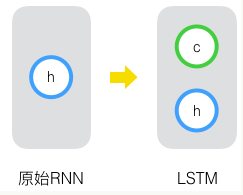
\includegraphics[scale=1]{1.png}
    \caption{cell}
    \label{fig:1}
\end{figure}

把上图按照时间维度展开:

\begin{figure}[H]
    \centering
    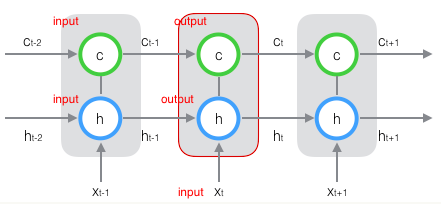
\includegraphics[scale=1]{2.png}
    \caption{cell}
\end{figure}

在 t 时刻,LSTM 的输入有三个:当前时刻网络的输入值 x\_t、上一时刻 LSTM 的输出值 h\_t-1、以及上一时刻的单元状态 c\_t-1;
LSTM 的输出有两个:当前时刻 LSTM 输出值 h\_t、和当前时刻的单元状态 c\_t.

\subsubsection{LSTM的前向计算}

\begin{enumerate}
    \item 遗忘门:它决定了上一时刻的单元状态 c\_t-1 有多少保留到当前时刻 c\_t
    \item 输入门:它决定了当前时刻网络的输入 x\_t 有多少保存到单元状态 c\_t
    \item 输出门:控制单元状态 c\_t 有多少输出到 LSTM 的当前输出值 h\_t
\end{enumerate}


\subsection{代码实现}

\begin{python}
    class LSTM(nn.Module):
    def __init__(self,input_size, hidden_size, num_layers,output_size,dropout_prob,directions = 1):
        super(LSTM,self).__init__()

        self.num_layers = num_layers
        self.hidden_size = hidden_size
        self.directions = directions

        self.lstm = nn.LSTM(input_size,hidden_size,num_layers,batch_first=True,dropout=dropout_prob)
        self.dropout = nn.Dropout(dropout_prob)
        self.linear = nn.Linear(hidden_size,output_size)

    def init_hidden_states(self, batch_size):
        state_dim = (self.num_layers * self.directions, batch_size, self.hidden_size)
        return (torch.zeros(state_dim).to(device), torch.zeros(state_dim).to(device))

    def forward(self, x, states):
        x = x.view(len(x),1,-1)
        x, (h, c) = self.lstm(x, states)
        out = self.linear(x)
        return out, (h, c)


n_hidden = 128
#rnn = RNN(n_letters, n_hidden, n_categories)


INPUT_SZIE = n_letters
DROPOUT = 0.2
DIRECTIONS = 1
NUM_LAYERS = 2
BATCH_SIZE = 5
OUTPUT_SIZE = n_categories
HIDDEN_SIZE = n_hidden
LEARNING_RATE = 0.0001
STATE_DIM = NUM_LAYERS * DIRECTIONS, BATCH_SIZE, HIDDEN_SIZE

lstm = LSTM(INPUT_SZIE,
    HIDDEN_SIZE,
    NUM_LAYERS,
    OUTPUT_SIZE,
    DROPOUT).to(device)

\end{python}


\subsection{训练结果}

训练结果如图\ref{fig:1}所示
\begin{figure}[H]
    \centering
    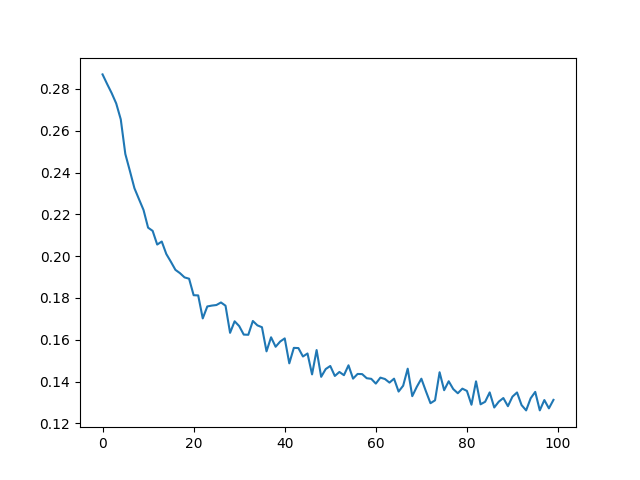
\includegraphics[scale=0.5]{myplot.png}
    \caption{训练结果}
    \label{fig:1}
\end{figure}

\section{解答}

LSTM 是为了解决 RNN 的 Gradient Vanish 的问题所提出的。关于 RNN 为什么会出 现 Gradient Vanish,上面已经介绍的比较清楚了,本质原因就是因为矩阵高次募导致的。下面简 要解释一下为什么 LSTM 能有效避免 Gradient Vanish。
对于 LSTM,有如下公式
$$
c^{t}=f^{t} \odot c^{t-1}+i^{t} \odot g^{t}
$$
模仿 RNN,我们来计算 $\delta^{k-1}=\partial C^{t} / \partial c^{k-1}$ ,有
$$
\begin{aligned}
\delta^{k-1} &=\frac{\partial C^{t}}{\partial c^{k-1}} \\
&=\frac{\partial C^{t}}{\partial c^{k}} \frac{\partial c^{k}}{\partial c^{k}-1} \\
&=\delta^{k} \frac{\partial c^{k}}{\partial c^{k-1}} \\
&=\delta^{k}\left(f^{t}+\ldots\right)
\end{aligned}
$$
公式里其余的项不重要,这里就用省略号代替了。可以看出当 $f^{t}=1$ 时,就算其余项很小,梯 度仍然可以很好导到上一个时刻,此时即使层数较深也不会发生 Gradient Vanish 的问题; 当 $f^{t}=0$ 时,即上-时刻的信号不影响到当前时刻,则梯度也不会回传回去; $f^{t}$ 在这里也控制 着梯度传导的㖜减程度,与它 Forget Gate 的功能一致。
%----------------------------------------------------------------

%----------------------------------------------------------------
\bibliographystyle{plain}
\end{document}
